\chapter{Appendix}
\label{chap:appendix_rapportclass}

\section{Rapports de classification combinés pour différentes méthodes}
\begin{table}[htbp]
    \centering
    \caption{Rapports de classification combinés pour différentes méthodes}
    \resizebox{\textwidth}{!}{%
    \begin{tabular}{@{}lccccccccc@{}}
    \toprule
    \textbf{Méthode} & \textbf{Dimensions des Features} & \multicolumn{2}{c}{\textbf{Classe 0}} & \multicolumn{2}{c}{\textbf{Classe 1}} & \textbf{Précision} & \textbf{Macro Moy.} & \textbf{Moy. Pondérée} \\
    & & \textbf{Précision} & \textbf{Rappel} & \textbf{Précision} & \textbf{Rappel} & & & \\
    \midrule
    comment\_text\_baseline & (63978, 52493) & 0.98 & 0.85 & 0.39 & 0.86 & 0.85 & (0.68, 0.86, 0.72) & (0.92, 0.85, 0.88) \\
    comment\_text\_bpe\_tokenize\_full\_normalization & (63978, 22188) & 0.98 & 0.86 & 0.40 & 0.87 & 0.86 & (0.69, 0.86, 0.73) & (0.93, 0.86, 0.88) \\
    comment\_text\_word\_tokenize\_no\_normalization & (63978, 52478) & 0.98 & 0.85 & 0.39 & 0.86 & 0.85 & (0.68, 0.85, 0.72) & (0.92, 0.85, 0.88) \\
    comment\_text\_gpt\_tokenize\_no\_normalization & (63978, 44632) & 0.97 & 0.90 & 0.45 & 0.74 & 0.89 & (0.71, 0.82, 0.75) & (0.92, 0.89, 0.90) \\
    comment\_text\_word\_tokenize\_normalization & (63978, 42934) & 0.98 & 0.85 & 0.39 & 0.87 & 0.85 & (0.69, 0.86, 0.73) & (0.93, 0.85, 0.88) \\
    comment\_text\_gpt\_tokenize\_normalization & (63978, 24578) & 0.98 & 0.87 & 0.40 & 0.80 & 0.86 & (0.69, 0.84, 0.73) & (0.92, 0.86, 0.88) \\
    comment\_text\_word\_tokenize\_full\_normalization & (63978, 41908) & 0.98 & 0.85 & 0.39 & 0.88 & 0.85 & (0.69, 0.86, 0.73) & (0.93, 0.85, 0.88) \\
    comment\_text\_gpt\_tokenize\_full\_normalization & (63978, 22750) & 0.98 & 0.86 & 0.40 & 0.85 & 0.86 & (0.69, 0.85, 0.73) & (0.92, 0.86, 0.88) \\
    comment\_text\_word\_tokenize\_simple\_normalization & (63978, 48335) & 0.98 & 0.85 & 0.39 & 0.86 & 0.85 & (0.68, 0.86, 0.72) & (0.92, 0.85, 0.88) \\
    comment\_text\_gpt\_tokenize\_simple\_normalization & (63978, 29389) & 0.98 & 0.86 & 0.39 & 0.82 & 0.86 & (0.69, 0.84, 0.72) & (0.92, 0.86, 0.88) \\
    comment\_text\_bpe\_tokenize\_simple\_dup\_normalization & (63978, 27126) & 0.98 & 0.86 & 0.39 & 0.85 & 0.86 & (0.69, 0.85, 0.73) & (0.92, 0.86, 0.88) \\
    comment\_text\_bpe\_tokenize\_no\_dup\_no\_punc\_normalization & (63978, 27290) & 0.98 & 0.86 & 0.39 & 0.85 & 0.86 & (0.69, 0.85, 0.73) & (0.92, 0.86, 0.88) \\
    \bottomrule
    \end{tabular}%
    }
    \end{table}

    \section{Matrice de confusion}
    \begin{figure}[ht]
        \caption{Matrice de confusion du modèle \textit{Bayésien naïf}}
        \centering
        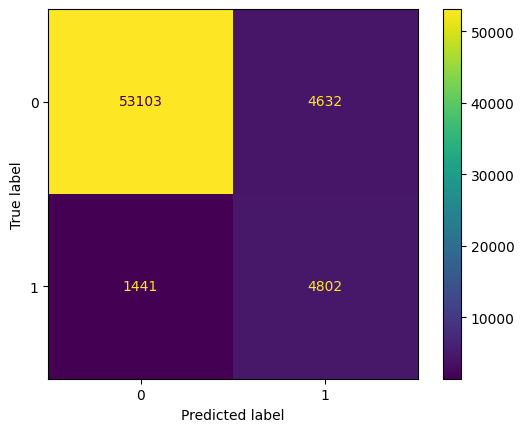
\includegraphics[width=.49\linewidth]{figures/matrix-confusion-naive_bayes.png}
    \end{figure}
\section{Distribution de la toxicité pour l'entraînement du modèle}
    \begin{figure}[ht]
        \caption{Distribution de la toxicité des commentaires}
        \centering
        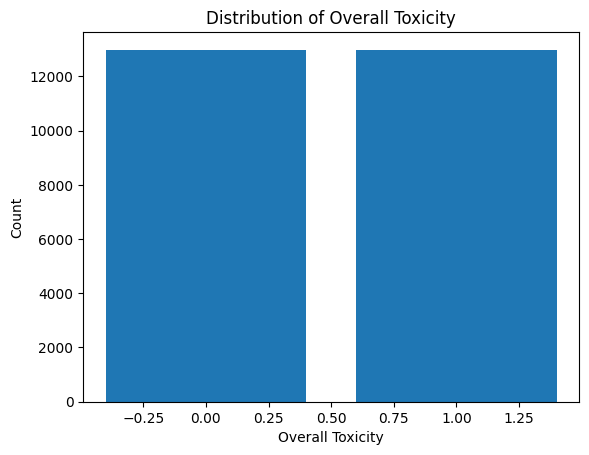
\includegraphics[width=.43\linewidth]{figures/distribution-toxicity-naive_bayes.png}
    \end{figure}
\section{Tableau des 30 mots non toxiques}
    \begin{figure}[htbp]
        \centering
        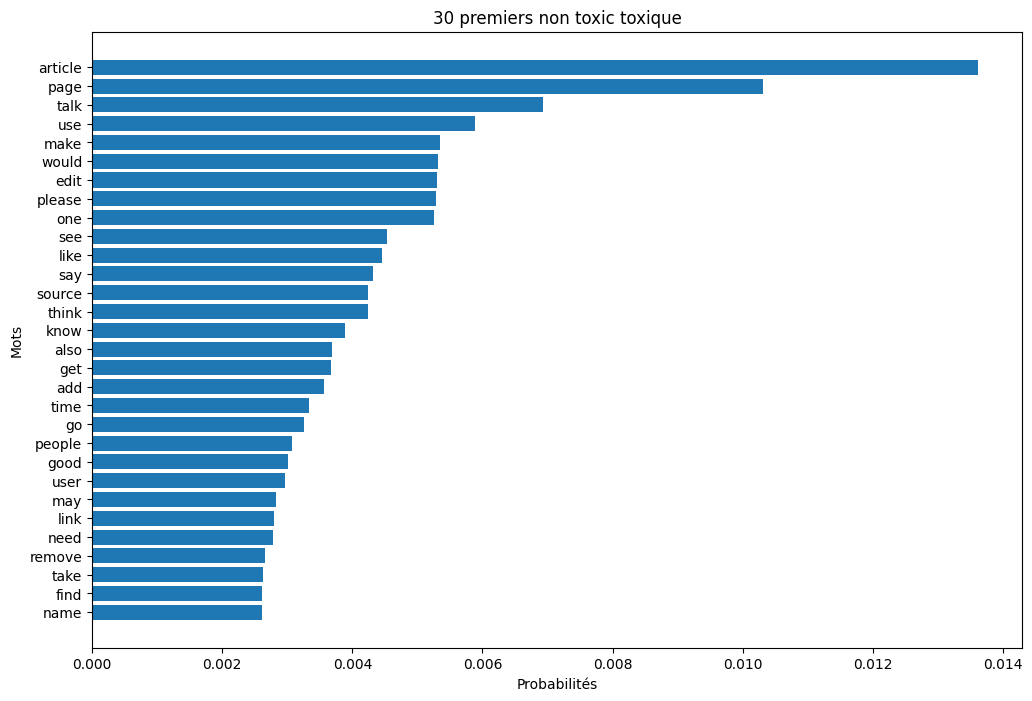
\includegraphics[width=.7\linewidth]{figures/30_first_non_toxic-naive_bayes.png}
        \caption{Top 30 mots non toxiques}
    \end{figure}
    \section{Tableau des 30 mots toxiques}
    \begin{figure}[htbp]
        \centering
        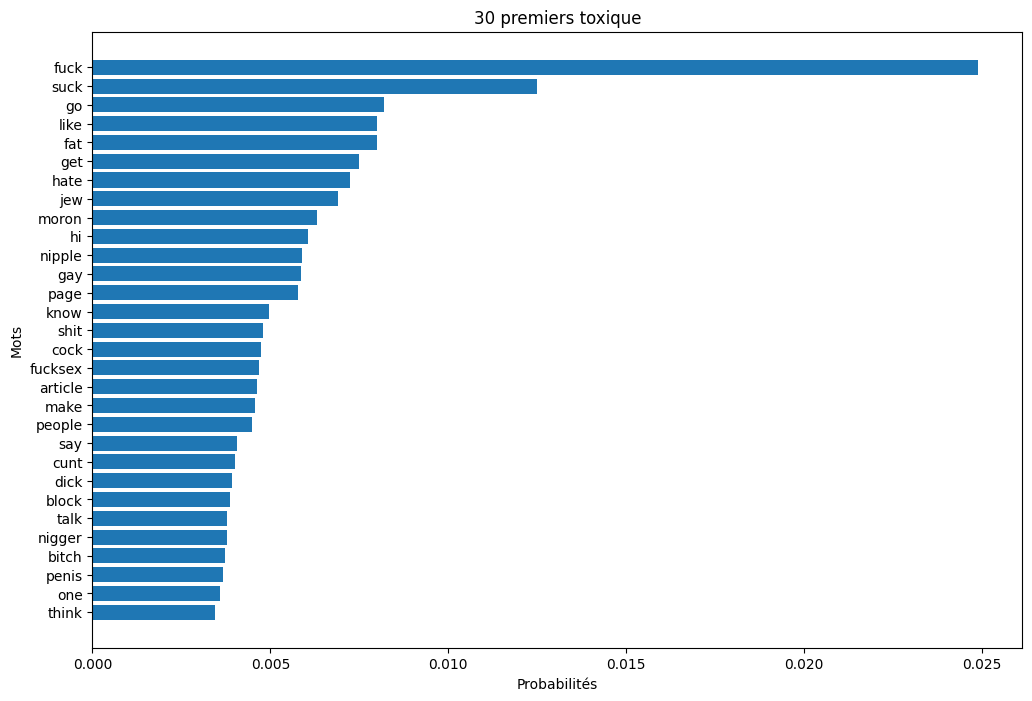
\includegraphics[width=.7\linewidth]{figures/30_first_toxic-naive_bayes.png}
        \caption{Top 30 mots toxiques}
    \end{figure}